%------------------------------------------------------------------------------------------------------------------------
\chapter{電荷補正の最適化}
\label{sec:chap4}
%------------------------------------------------------------------------------------------------------------------------
Thresholdのチューニングおよび電荷較正を行った後、それぞれのパラメータが適切な値を保持していることを確認しデータベースに必要なパラメータ情報の登録を行う。ピクセルモジュールの電荷較正では正しく結果を出力しない場合があるため、電荷較正結果に適切な値を補完しデータベースにアップロードする必要がある。電荷較正の際に発生するいくつかの問題に対し、例外処理を行いより適切な値に近い値を補完するアルゴリズムの開発を行った。
本章では、電荷較正で発生する問題と、その問題に対する処理方法について説明する。

%------------------------------------------------------------------------------------------------------------------------
\section{電荷較正における補正の概要}
\label{sec:hoseigaiyou}
%------------------------------------------------------------------------------------------------------------------------

電荷較正では、ピクセル検出器およびIBLに搭載された計28400個のFEチップを同時に操作するため、全てが正常に機能しないことがある。電荷較正における問題は主に以下の2つがあげられる。
%本節ではそれぞれについての問題の原因とこれまでの補完方法について説明する。

\begin{itemize}
  \item[1. ] 不適当な電荷を使った電荷較正
  \item[2. ] データの欠陥
\end{itemize}

1つ目の問題に関して、ピクセルモジュールの電荷較正ではFEチップに搭載された回路を用いて試験電荷を生成し、ThresholdスキャンやToTスキャンを行う。電荷生成のための回路のいずれかの部分に故障等の問題があると、誤った試験電荷を生成してしまう。問題がある場合とない場合の試験電荷について、電荷較正\eref{eq:calibration}を用いてフィッティングした結果を\fref{fig:calibhikaku}に示す。\fref{fig:calibhikaku}において、左図は理想的なフィッティング結果を表しており、全ての点がフィット曲線上に乗っていることがわかる。この様に、ToTとセンサーが落とす電荷量は、おおよそ線形関係にあることがわかる。

\begin{figure}[tbp]
  \begin{minipage}[b]{0.5\linewidth}
    \centering
    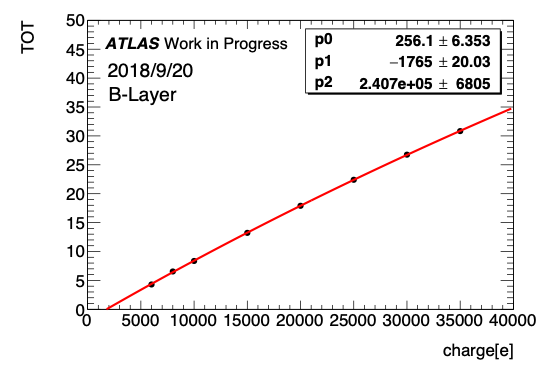
\includegraphics[keepaspectratio, scale=0.8]{goodcalib.png}
  \end{minipage}
  \begin{minipage}[b]{0.5\linewidth}
    \centering
    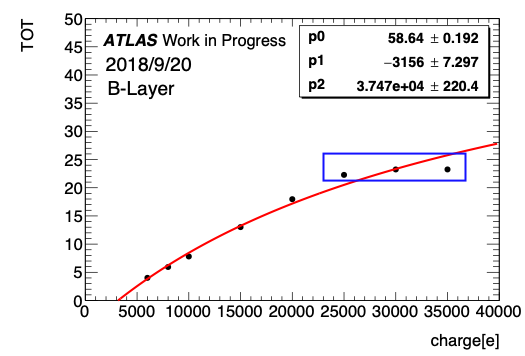
\includegraphics[keepaspectratio, scale=0.8]{badcalib.png}
  \end{minipage}
  \caption[電荷較正\eref{eq:calibration}を用いてフィッティングした結果]{電荷較正\eref{eq:calibration}を用いてフィッティングした結果。左図は理想的なフィッティング結果を表しており、右図は正しいToTが得られていない点を含むフィッティング結果である。}
  \label{fig:calibhikaku}
\end{figure}

一方で、右図は電荷生成の回路に問題のあるFEチップにおける電荷較正結果であり、電荷量の大きい3つの試験電荷についてToTの値がほとんど同じ値になっている。この原因は、試験電荷生成のための回路における電圧$V_\mathrm{cal}$の生成機構にある。$V_\mathrm{cal}$は\textbf{Plsr DAC}と呼ばれる$10\ \si{bit}$の値により決定される。$V_\mathrm{cal}$と$\mathrm{Plsr\ DAC}$の関係は\eref{eq:vcal}のように、1次式で与えられる。
\begin{equation}
  \label{eq:vcal}
  V_\mathrm{cal} = a + b\ (\mathrm{Plsr\ DAC})\ [\si{mV}]
\end{equation}
ここで、$a,\ b$は較正によって決定される定数であり、FEチップごとに個体差がある。あるFEチップに対する$V_\mathrm{cal}$とPlsr DACの関係の測定結果を\fref{fig:vcalplot}に示す。この図において、$\mathrm{Plsr\ DAC}\approx 750$までは$V_\mathrm{cal}$とPlsr DACの値が線形となっているが、それ以降のPlsr DAC値においては$V_\mathrm{cal}$が飽和していることがわかる。この$V_\mathrm{cal}$の飽和は、試験電荷生成回路におけるキャパシタ$C_\mathrm{low}$および$C_\mathrm{high}$の内、$C_\mathrm{low}$のみを用いて試験電荷を生成した場合に発生しやすいことがわかっている \cite{houwa}。\fref{fig:analog}に示したように、$C_\mathrm{high}$の前に配置されているスイッチを用いる事により使用するキャパシタの選択を行うことができる。電荷較正の際には、$C_\mathrm{low}$のみを用いるためこのスイッチは開放されているが、$V_\mathrm{cal}$の値が大きいときにはグランドへのリーク電流が大きくなってしまう。そのため、ある値以上の電荷を持つ試験電荷を正確に取得することができず、正しい電荷較正結果が得られない。$V_\mathrm{cal}$の飽和が起きていると予想される\fref{fig:calibhikaku}の右図の場合は、電荷較正に使用された試験電荷の内、正しいToTが得られていない2点を取り除き、再較正を行う必要がある。
\begin{figure}[tbp]
  \centering
  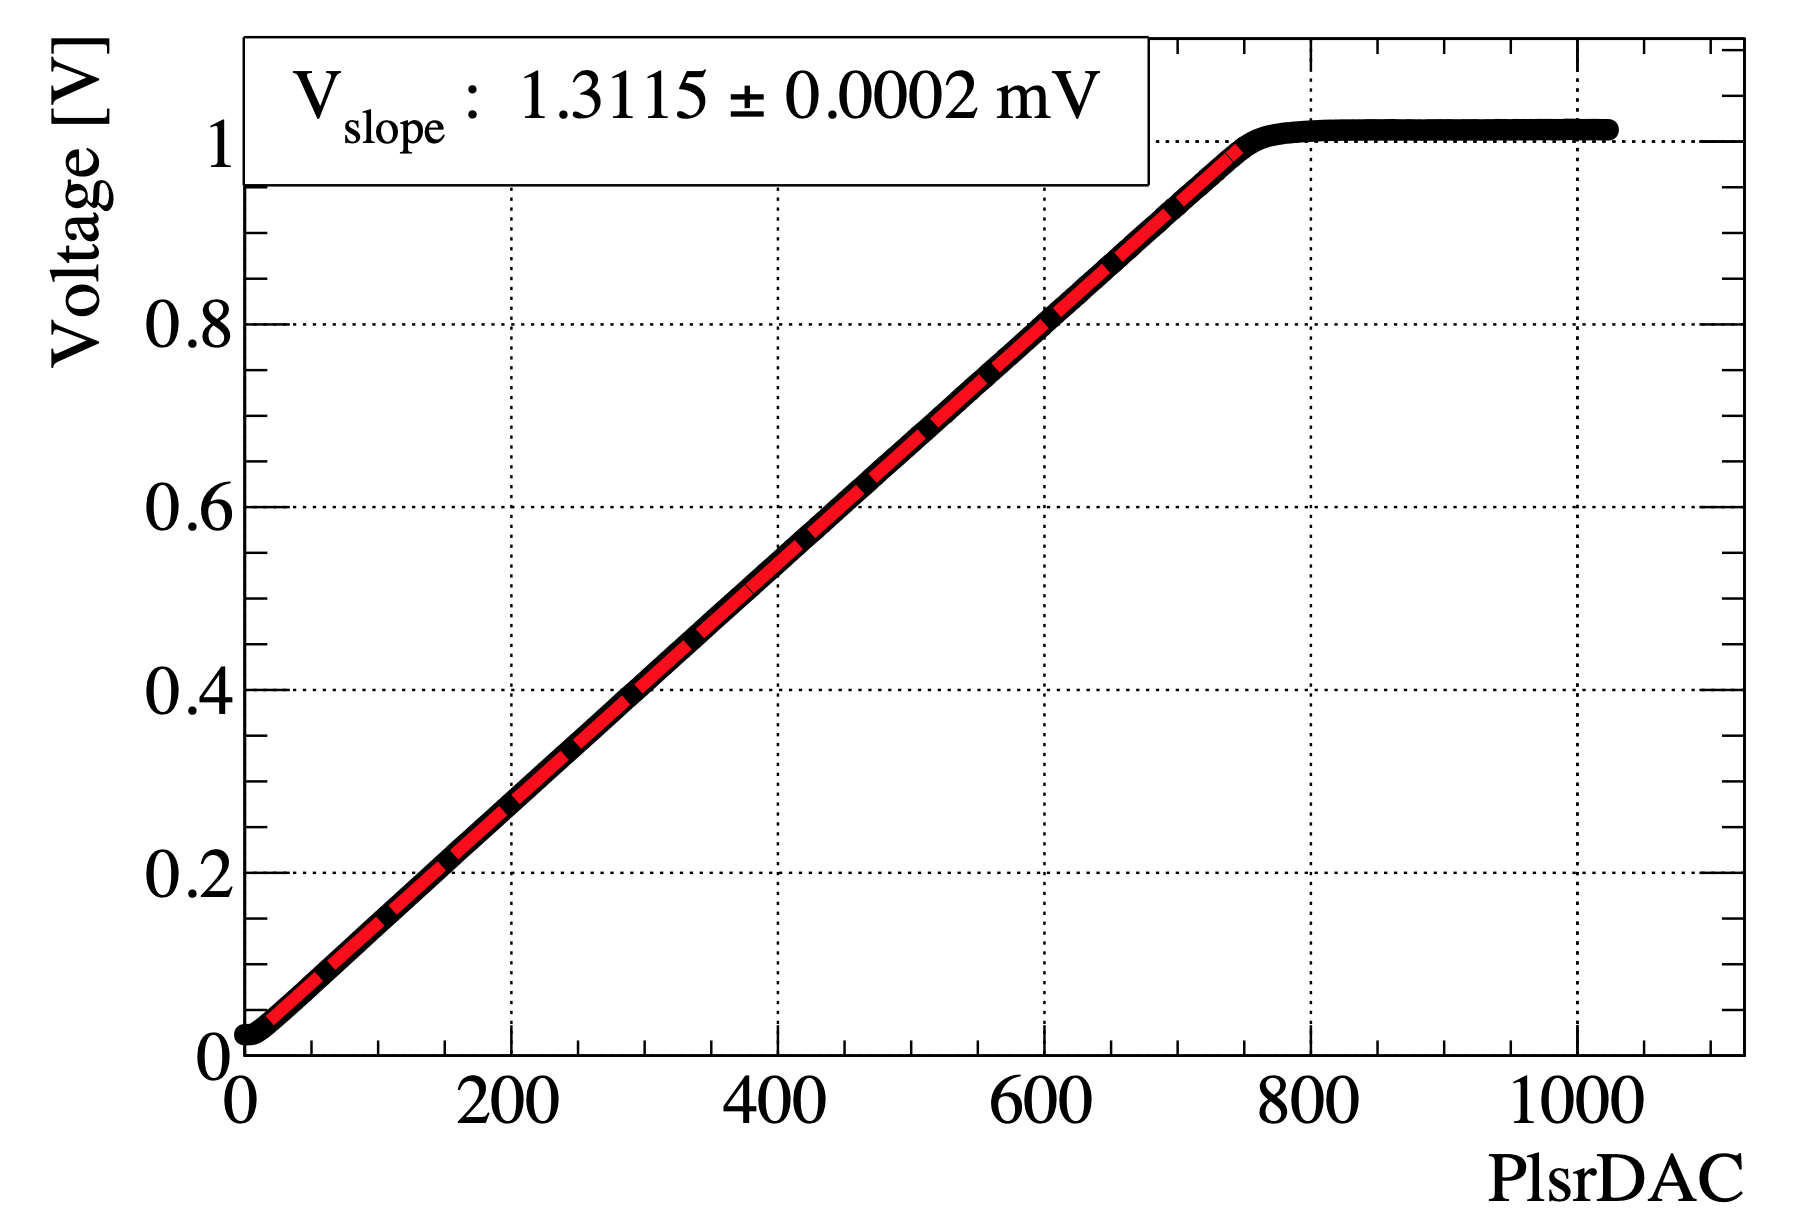
\includegraphics[height=7cm,keepaspectratio]{vcalplsr.png}
  \caption[$V_\mathrm{cal}$とPlsr DACの関係の測定結果]{$V_\mathrm{cal}$とPlsr DACの関係の測定結果 \cite{vcal}。黒点は各Plsr DACに対する$V_\mathrm{cal}$の測定点を表し、赤線は\eref{eq:vcal}を用いたフィッティング結果である。図中における$V_\mathrm{slope}$は赤線の傾きであり、\eref{eq:vcal}における$b$に対応する。}
  \label{fig:vcalplot}
\end{figure}

2つ目の問題に関して、あるFEチップに対してスキャンが失敗してしまった時にデータが欠陥してしまうことがある。あるピクセルモジュールについて全てのデータが欠陥してしまっている場合には、直前に行われた電荷較正結果をコピーすることにより補完を行う。また、ピクセルモジュールにおいてデータの一部が欠陥してしまっている場合は最も近いFEチップから値をコピーすることにより補完を行う。ピクセルモジュールの一部のFEチップに欠陥が含まれるThresholdの分布を\fref{fig:thresholdkekkan}に示す。\fref{fig:thresholdkekkan}の場合は、ピクセルモジュールに搭載された16個のFEチップの内の1つ(図中のI6の部分)についてのThreshold値が欠陥しており、値が全て0となっている。このように一部のみにデータの欠陥が見つかった場合は、最も近いFEチップ(\fref{fig:thresholdkekkan}の場合はI5、I7、I9のいずれか1つ)から値をコピーすることによって補完作業を行っていた。

\begin{figure}[tbp]
  \centering
  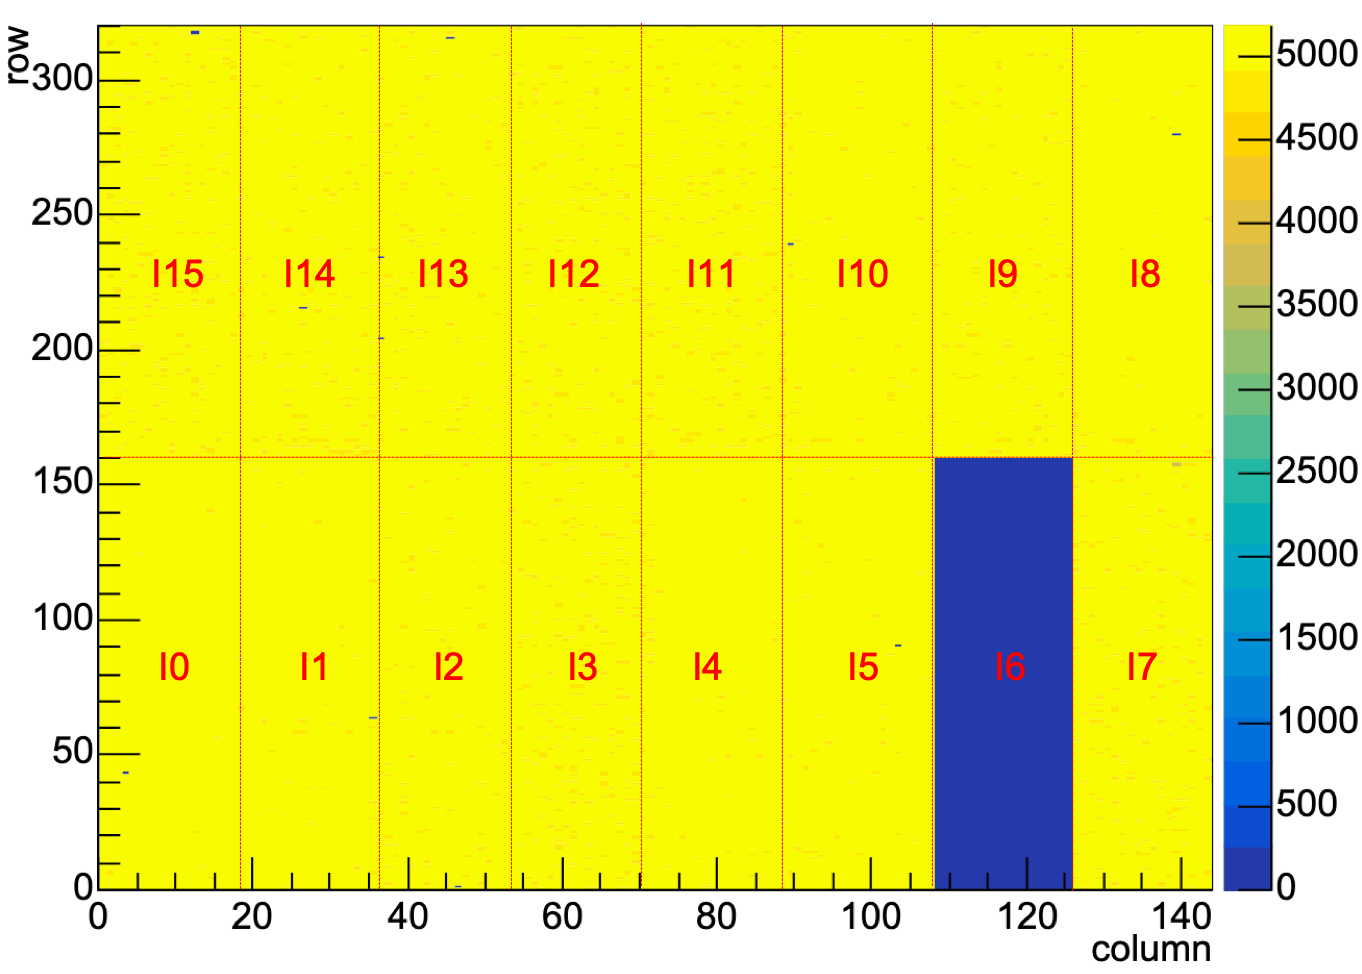
\includegraphics[height=7cm,keepaspectratio]{thresholdkekkan.png}
  \caption[欠陥が含まれるピクセルモジュールについてのThreshold分布]{欠陥が含まれるピクセルモジュールについてのThreshold分布。この図のように、Thresholdスキャンの結果はモジュールごとに出力され、行と列の領域によりFEチップの識別を行うことができる。}
  \label{fig:thresholdkekkan}
\end{figure}

%------------------------------------------------------------------------------------------------------------------------
\subsection{これまでの電荷較正の再補正}
\label{sec:prehosei}
%------------------------------------------------------------------------------------------------------------------------

ATLASに搭載されたピクセル検出器およびIBLのピクセルモジュールについて電荷較正を行うが、測定を行っていると放射線損傷の影響によって、補正値がずれてしまう。\fref{fig:thresholdhennka}にRUN2におけるIBLのMIP粒子に対するToTの推移を示す。
このToTの推移はセンサーがトータルドーズ効果による放射線損傷を受けることによるものである。
放射線損傷が小さい場合(TID $\leq1$-$6\ [\si{Mrad}]$)、FEチップ電流は増加する。そのため、実行的なThreshold値が大きくなり、MIP粒子に対するToTは小さくなる(\fref{fig:thresholdhennka}の上図)。
一方で、放射線損傷が大きい場合(TID $\geq1$-$6\ [\si{Mrad}]$)、FEチップ電流は小さくなる。そのため、実行的なThreshold値が小さくなり、ToTの値は大きくなる(\fref{fig:thresholdhennka}の下図)。

%トータルドーズ効果とセンサーの漏れ電流の関係を\fref{fig:totaldoze}示す。

%IBLではMIP粒子がセンサーに落とす電荷量は$16\ \si{ke}$であるが、
このように、放射線損傷を受けることによりToTの値が目標値である$10\ \si{ToT}$から変化していることがわかる。目標値からのずれを補正するため、2018年における電荷較正は2週間から4週間の周期で行っており、電荷較正の後には\ref{sec:hoseigaiyou}節で説明した問題を取り除くため、補完作業を行う必要がある。

\begin{figure}[tbp]
  \centering
  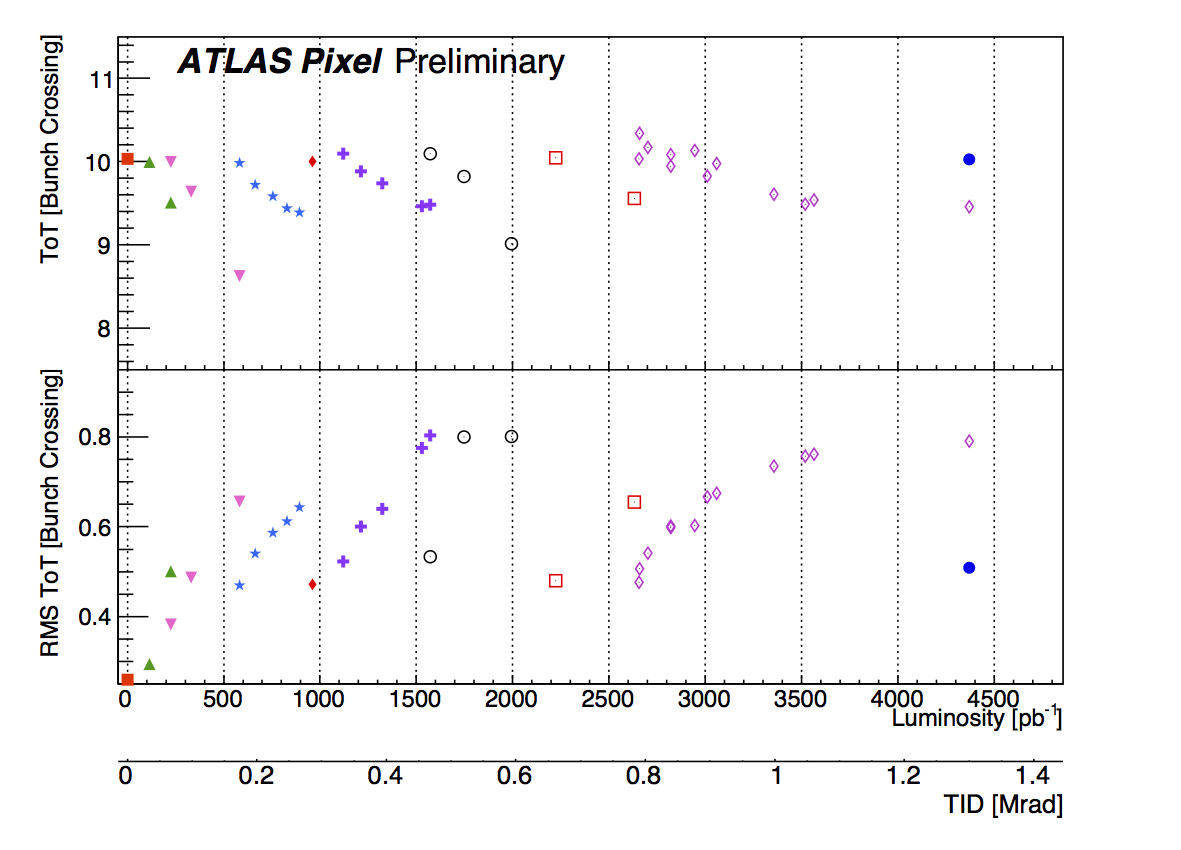
\includegraphics[height=7.8cm,keepaspectratio]{tothennkarow.png}
  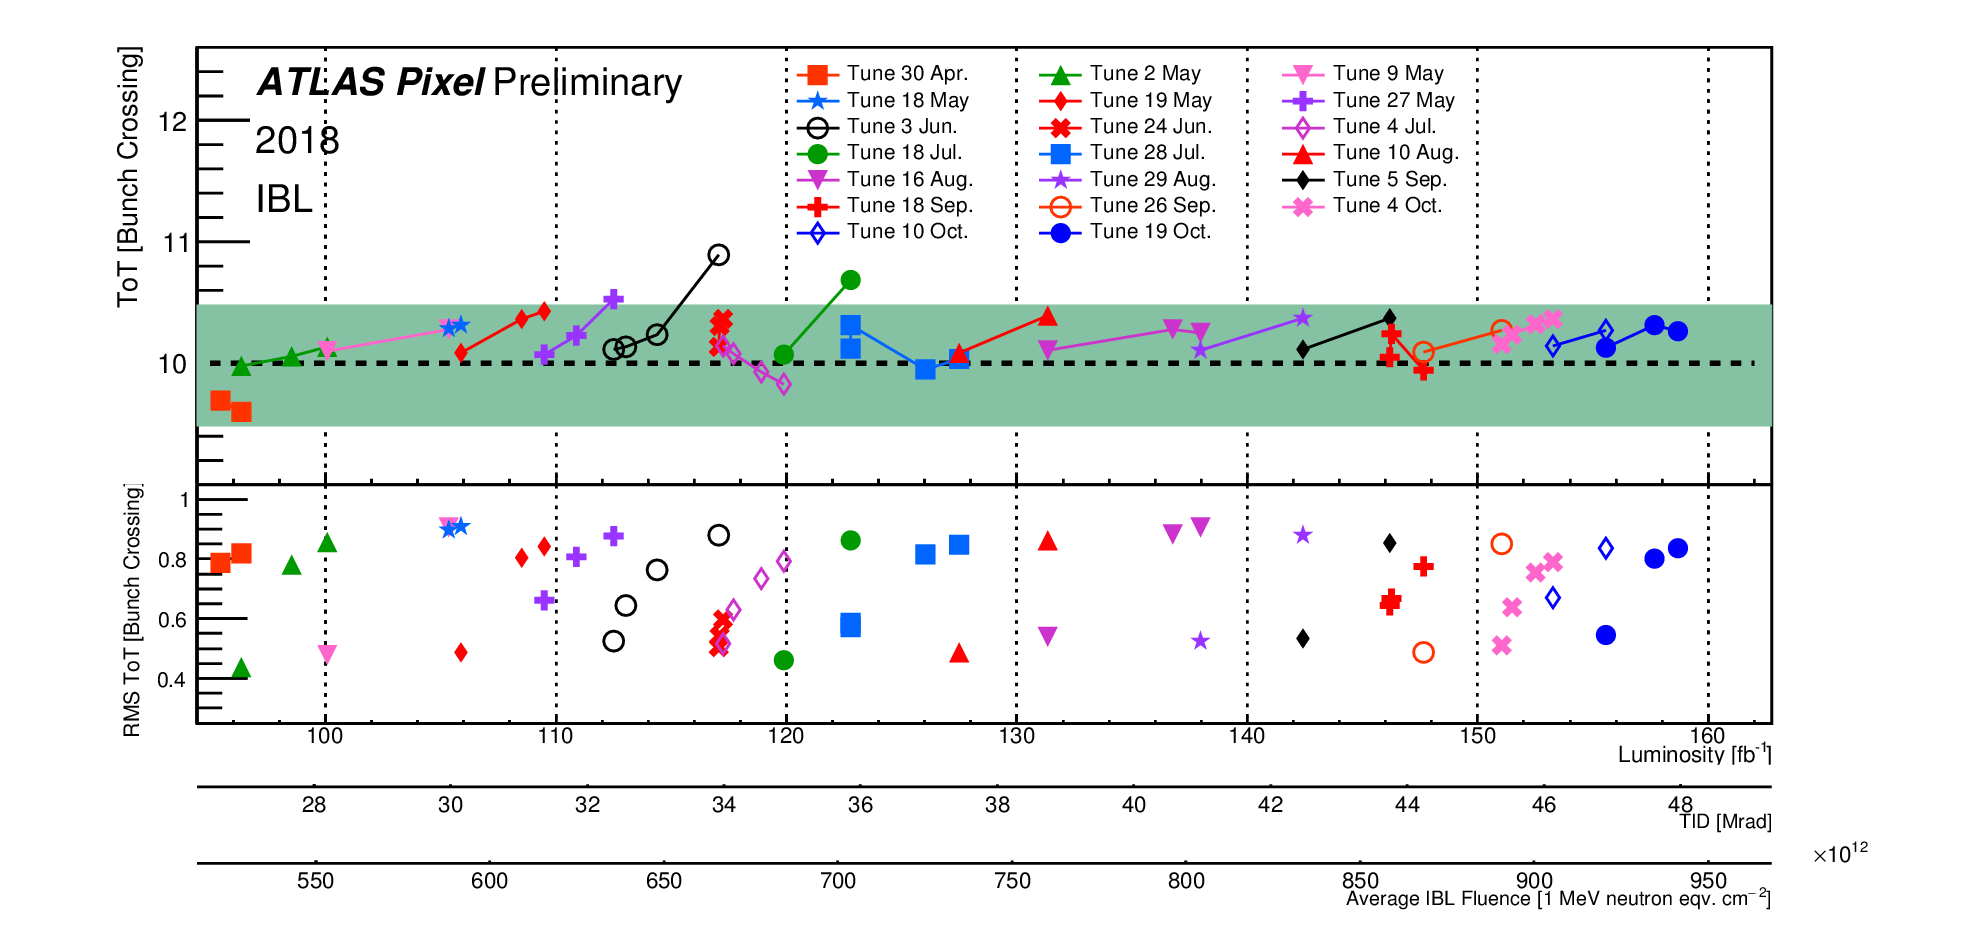
\includegraphics[height=7.5cm,keepaspectratio]{tothennka.png}
  \caption[ルミノシティに対するToTの変化]{IBLのルミノシティに対するToTの変化 。上図は2015年におけるToTの変化\cite{tothenkarow}であり、左端はRun2開始時を表す。下図は2018年におけるToTの変化\cite{tothennka}で右端はRun2の最後を表す。IBLのToTの目標値は$16\ \si{ke}$の電荷量に対して$10\ \si{ToT}$であるが、トータルドーズ効果の影響を受け目標値からずれてしまう。}
  \label{fig:thresholdhennka}
\end{figure}


%\begin{figure}[tbp]
%  \begin{minipage}[b]{0.5\linewidth}
%    \centering
%    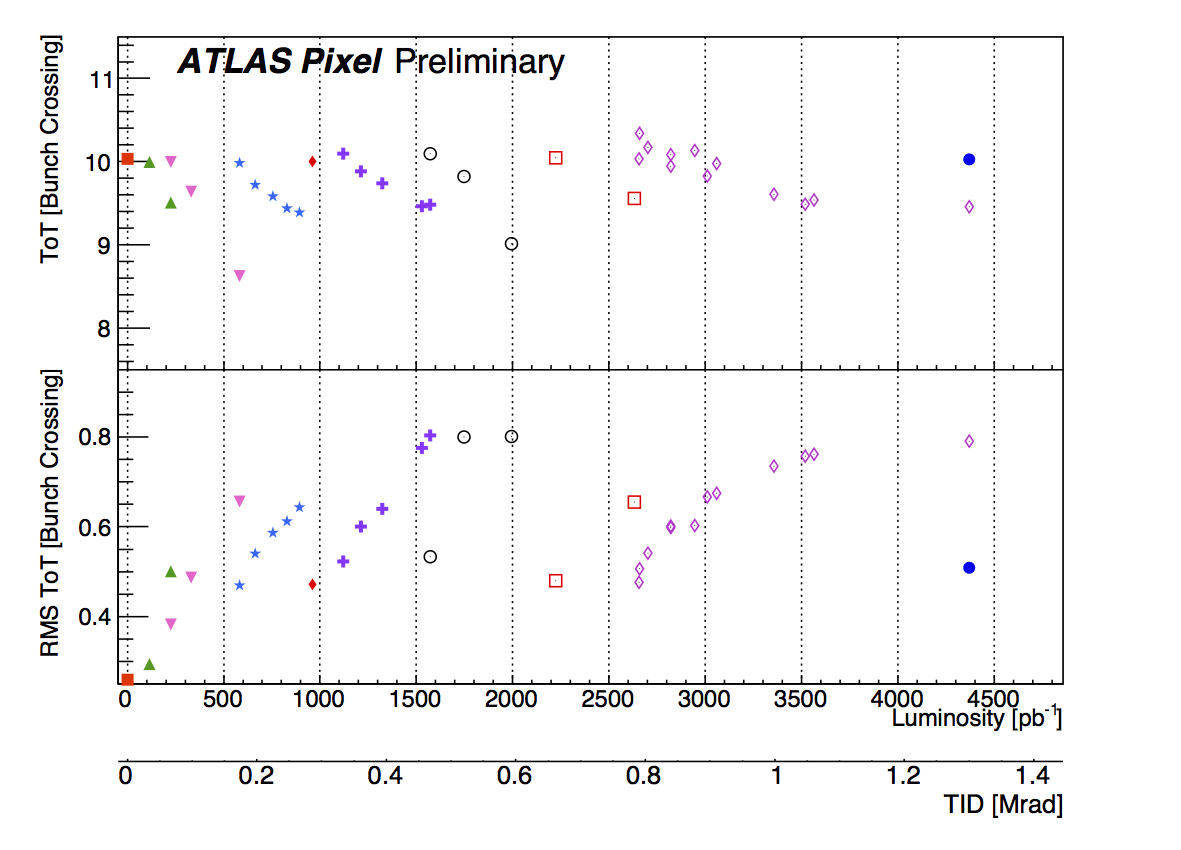
\includegraphics[keepaspectratio, scale=0.4]{tothennkarow.png}
%  \end{minipage}
%  \begin{minipage}[b]{0.5\linewidth}
%    \centering
%    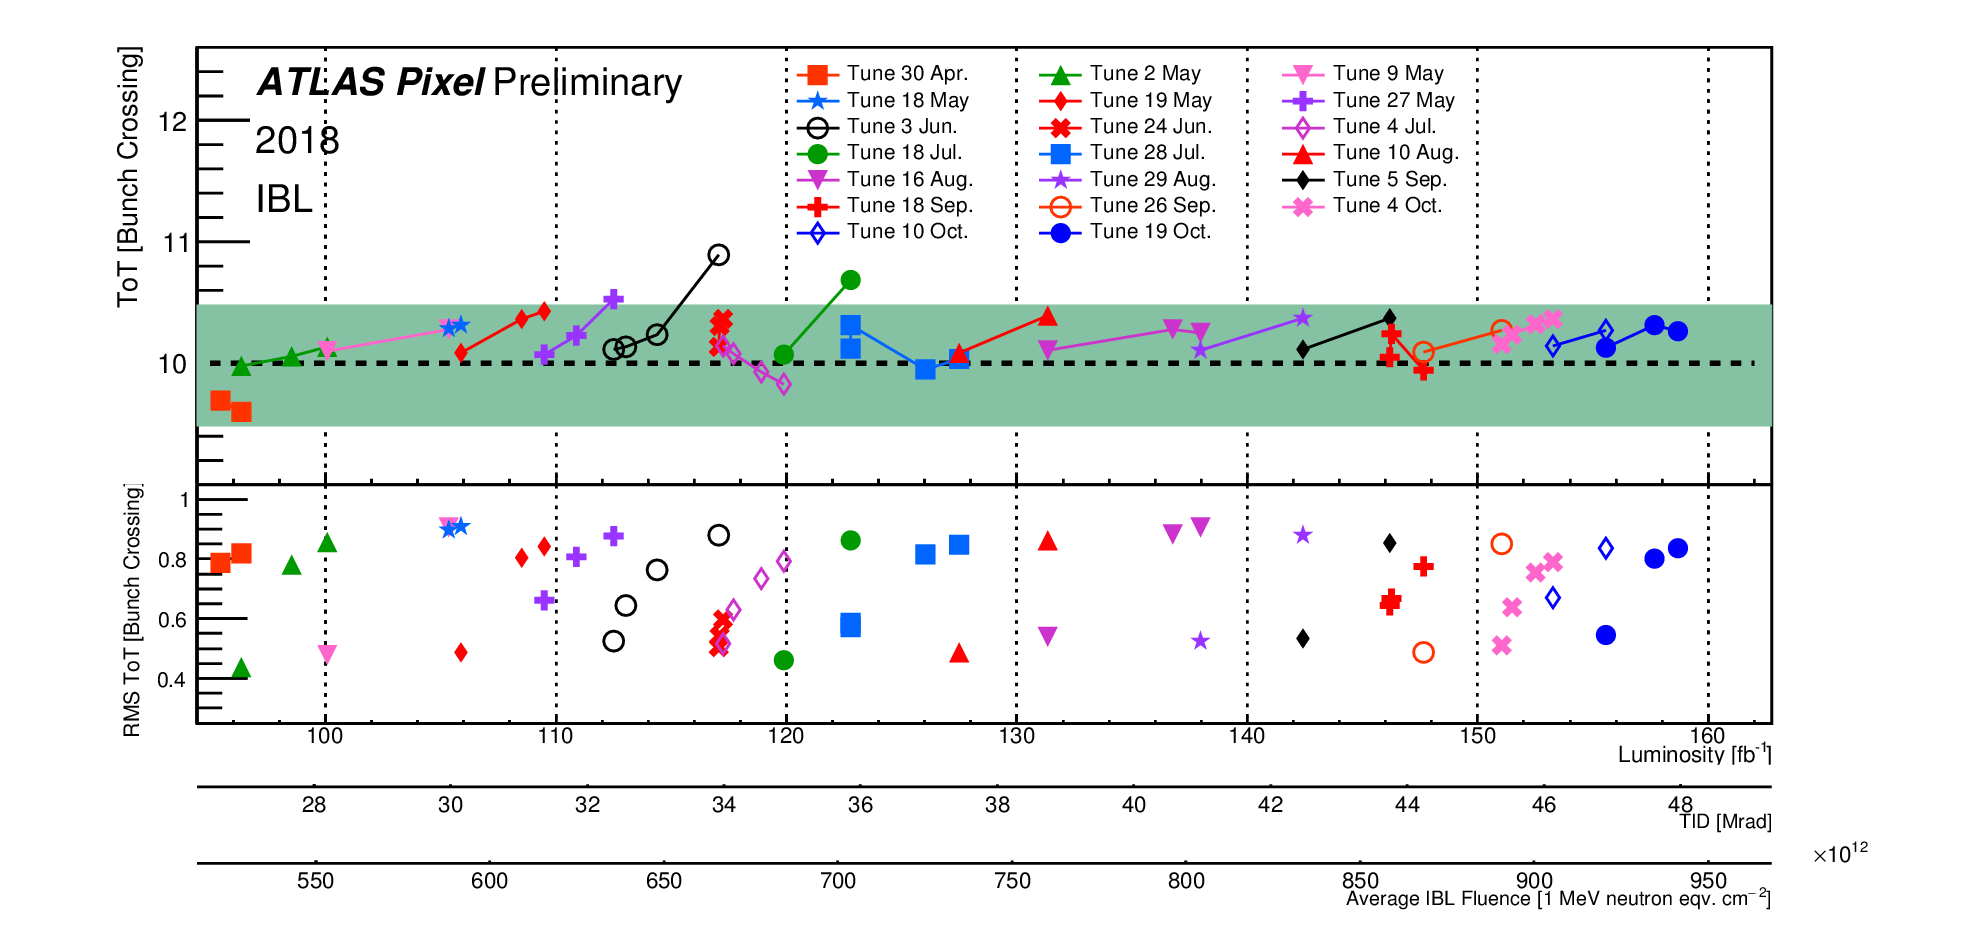
\includegraphics[keepaspectratio, scale=0.2]{tothennka.png}
%  \end{minipage}
%  \caption[ルミノシティに対するToTの変化]{ルミノシティに対するToTの変化}
%  \label{fig:calibhikaku}
%\end{figure}

%\begin{figure}[tbp]
%  \centering
%  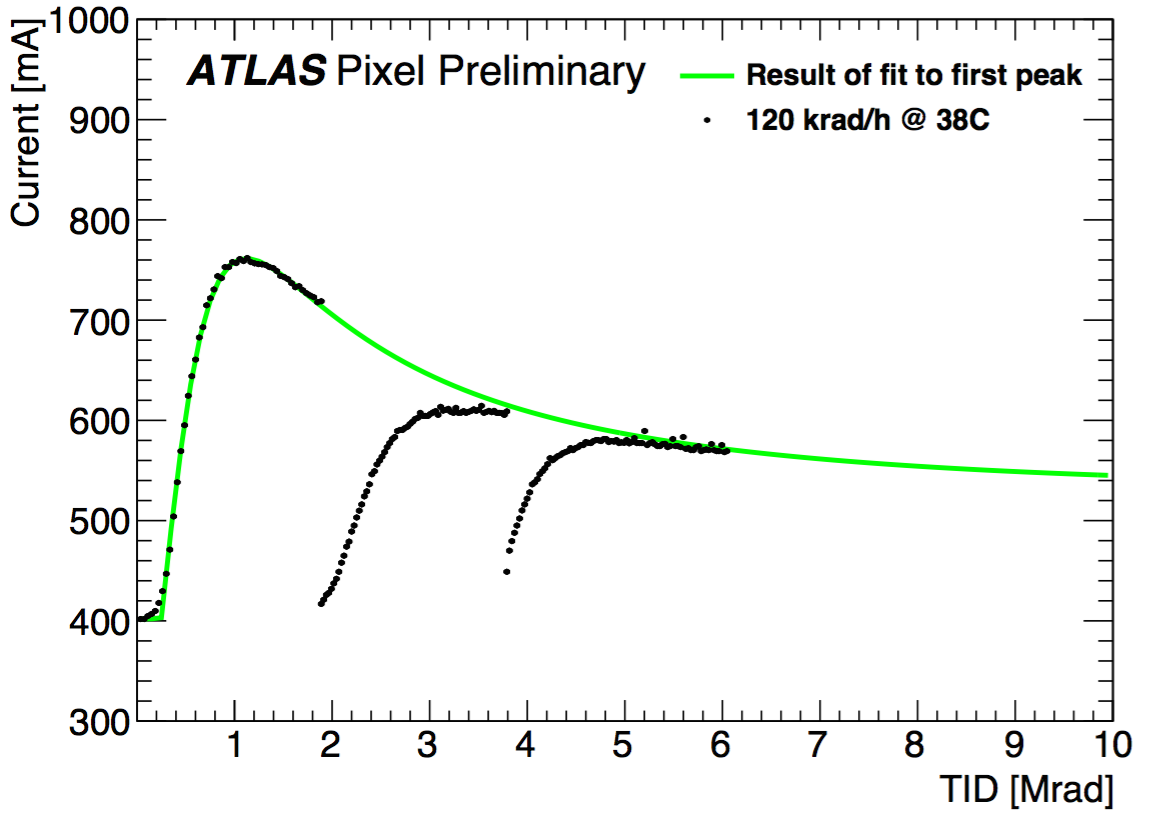
\includegraphics[height=7.5cm,keepaspectratio]{totaldose.png}
%  \caption[トータルドーズ効果と漏れ電流の関係]{トータルドーズ効果と漏れ電流の関係 \cite{totaldoze}。}
%  \label{fig:totaldoze}
%\end{figure}


これまで、電荷較正後の補完作業は1人の担当者による手作業で行われていた。RUN3からは放射線損傷による影響がさらに大きくなることから、電荷較正の頻度が10日に1度程度になる予定であり、この作業を行うのは非常に労力が伴う。さらに、これまで行っていた補正では手作業による補正であることから、担当者によっては異なる値を補完してしまうことがある。本研究では適切な欠損の補完処理を行うよう、例外をアルゴリズムとして抽出・処理する自動解析ツールの開発を行った。次節からそれについて説明する。


%------------------------------------------------------------------------------------------------------------------------
\section{電荷較正の補正}
\label{sec:calibhosei}
%------------------------------------------------------------------------------------------------------------------------
\fref{fig:calibhikaku}の右図に示すように、電荷生成のための回路の個体差により正しい電荷が生成できず、誤ったToTを持つ電荷を用いて電荷較正を行ってしまう場合がある。この様な点を取り除くために、これまでは\eref{eq:averagedistance}を用いて電荷較正結果の評価を行っていた。
\begin{equation}
  \label{eq:averagedistance}
  \Delta d = \sum_{i=1}^{N} \frac{ToT_{true, i} - ToT_{fit, i}}{N}
\end{equation}
ここで、$N$は電荷較正に使われた試験電荷の数であり、$ToT_{true, i}$および$ToT_{fit, i}$はそれぞれ電荷較正に使用された$i$番目のToTおよび電荷較正式によるフィッティングから得られる$i$番目のToTである。
%電荷較正結果の評価のために、全てのFEチップにおいて計算した$\Delta d$の分布を\fref{fig:averagedistance}に示す。
この評価では$\Delta d > 0.5$の場合、電荷較正に正しく生成されいない試験電荷が存在するとし、そのフィッティング結果を取り出して補正を行っており、2018年9月における電荷較正では、約250個の正しく電荷が生成されていないフィッティング結果が見つかり、その補正を行った。

%\begin{figure}[tbp]
 % \centering
 % 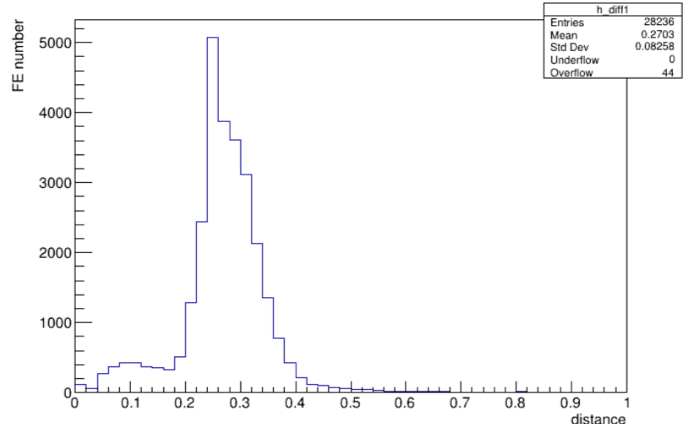
\includegraphics[height=6cm,keepaspectratio]{averagedistance.png}
 % \caption[電荷較正結果の評価のための$\Delta d$の分布]{電荷較正結果の評価のための$\Delta d$の分布。}
%  \label{fig:averagedistance}
%\end{figure}

\eref{eq:averagedistance}の評価方法は、電荷較正に使う試験電荷の数によって大きさが変化するものである。そのため、問題のある試験電荷を取り除いた後の電荷較正結果の評価のための基準値は、$0.5$とは別の値を用いる必要がある。自動補正を行う際、電荷再較正を行う度に基準値を変更するのは非常に困難である。
そこで、本研究で新たな評価基準を導入し、それを用いた電荷再較正の自動化アルゴリズムの開発を行った。


%------------------------------------------------------------------------------------------------------------------------
\subsection{電荷較正結果の評価方法}
%------------------------------------------------------------------------------------------------------------------------
電荷較正結果を評価するための新たな基準を以下に示す。
\begin{itemize}
  \item[]\textbf{試験電荷とから得られる電荷の差が、試験電荷の5\%以上であれば問題のある試験電荷とする}
\end{itemize}
上記の評価基準は、ピクセル検出器における主な測定対象であるMIP粒子の検出感度から決定した。MIP粒子がピクセル検出器に落とす電荷量の分布を\fref{fig:mipdist}に示す。

\begin{figure}[tbp]
  \centering
  \includegraphics[height=7cm,keepaspectratio]{mipdist.png}
  \caption[MIP粒子がピクセル検出器に落とす電荷量]{MIP粒子がピクセル検出器に落とす電荷量。}
  \label{fig:mipdist}
\end{figure}

上記の基準を満たしていれば、MIP粒子がシリコンセンサーに落とす電荷の測定精度$5\%$であり、電荷較正による分解能が\fref{fig:mipdist}におけるランダウ分布の揺らぎより十分小さくできる。

また、この基準は各試験電荷について個別の評価を行っているため、試験電荷の数に依存せず電荷再較正の自動処理により適した評価方法である。\fref{fig:partialdistance}にB-Layerの全FEチップについて計算した試験電荷と電荷較正結果から得られる電荷の差の分布を示す。この分布において、試験電荷とから得られる電荷の差と試験電荷の比が$5\% $より大きいFEチップについて電荷較正結果の補正を行う。次項において、電荷再較正の処理方法について説明する。

\begin{figure}[tbp]
  \centering
  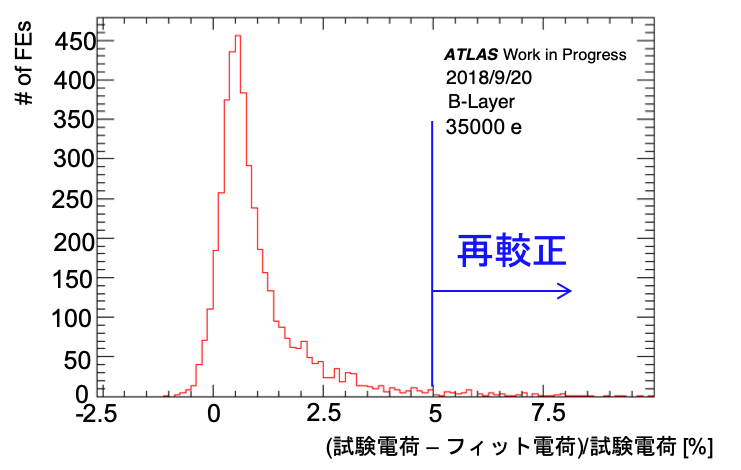
\includegraphics[height=7cm,keepaspectratio]{partialdistance.png}
  \caption[B-Layerの全FEチップについて計算した試験電荷と電荷較正結果から得られる電荷の差の分布]{B-Layerの全FEチップについて計算した試験電荷と電荷較正結果から得られる電荷の差の分布。}
  \label{fig:partialdistance}
\end{figure}


%------------------------------------------------------------------------------------------------------------------------
\subsection{電荷再較正の自動化アルゴリズム}
%------------------------------------------------------------------------------------------------------------------------
上記の評価基準を用いて電荷再較正を自動で行うツールを作成した。解析処理を行うために、CERNが提供している解析フレームワークであるROOTを使用している。電荷較正のために作成されたROOTの解析ツールを改良し、電荷較正後に結果の評価および再較正を行うプログラムを追加した。
作成したツールの処理の流れを\fref{fig:saikouseiflow}に示す。

\begin{figure}[tbp]
  \centering
  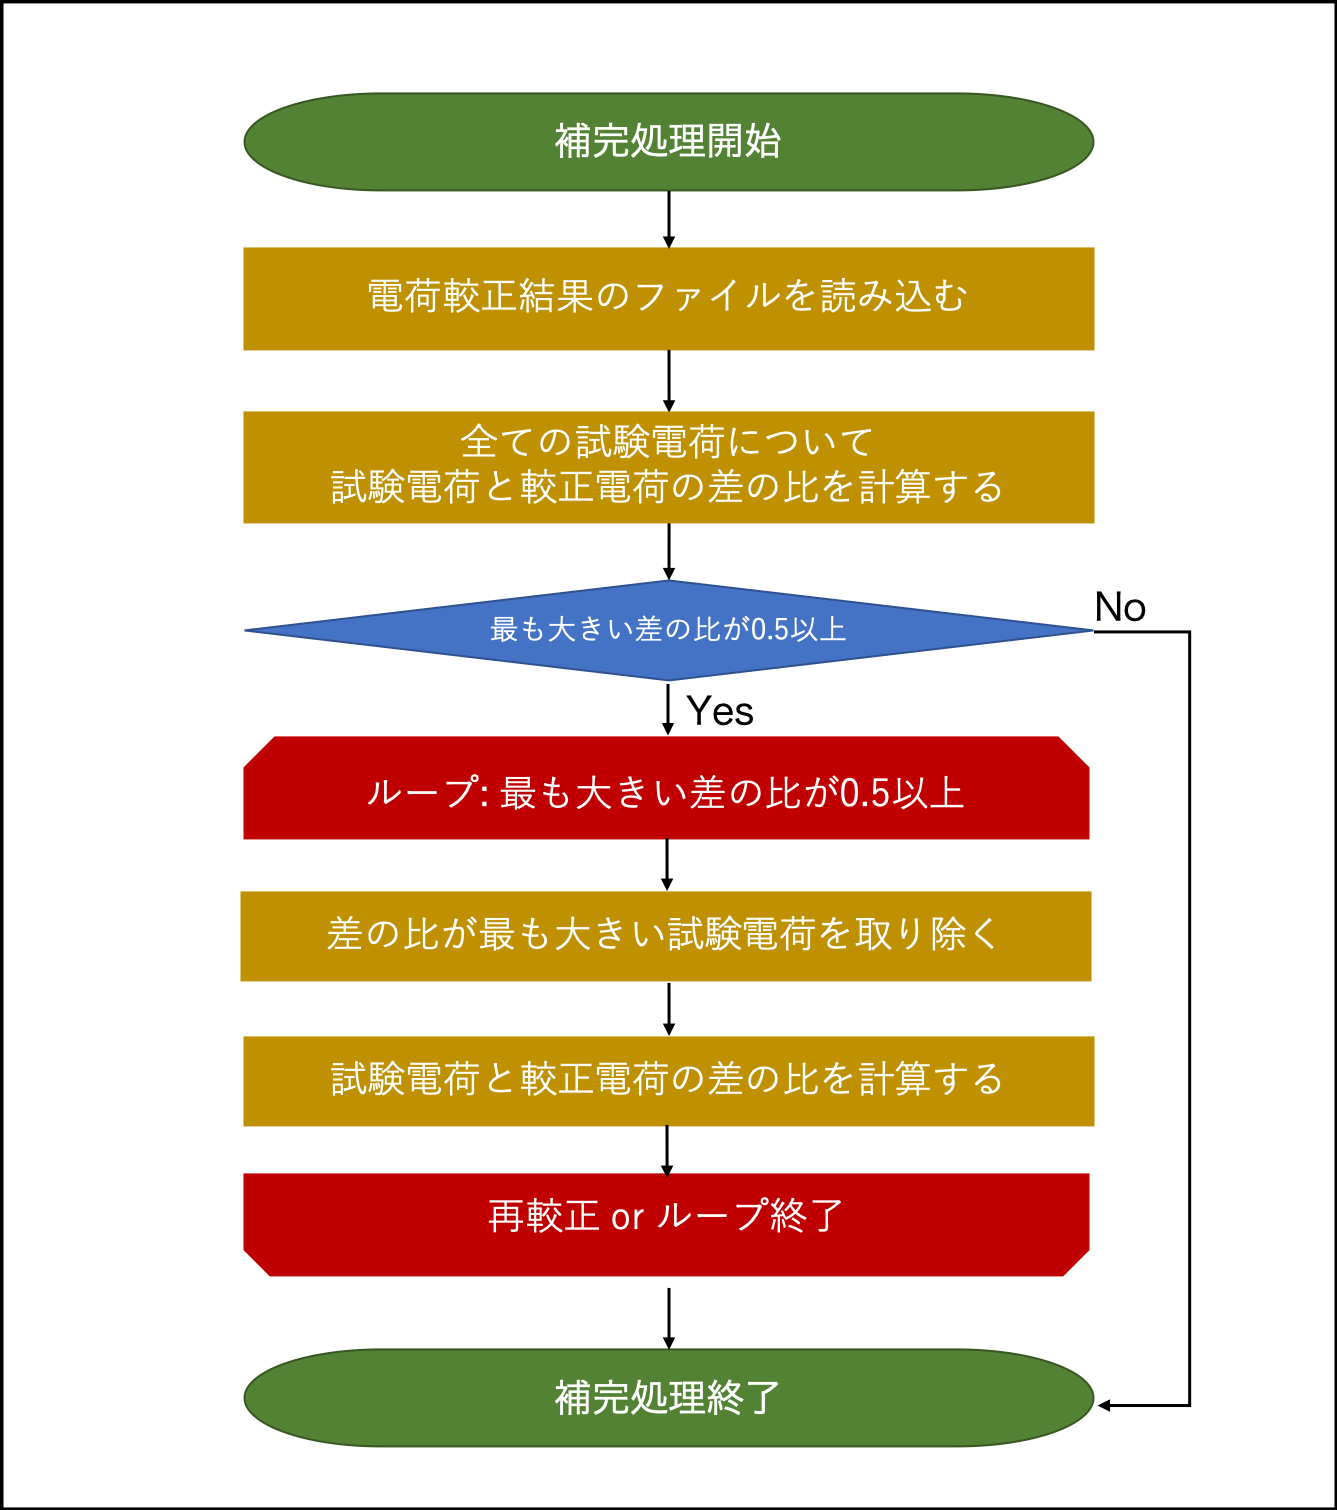
\includegraphics[height=10cm,keepaspectratio]{saikouseiflow.png}
  \caption[電荷較正結果を再較正するツールの処理の流れ]{電荷較正結果を再較正するツールの処理の流れ。}
  \label{fig:saikouseiflow}
\end{figure}


\fref{fig:saikouseiflow}に示したループの処理で電荷較正から得られる電荷と試験電荷の差が0.5\% 以内に収束するまで再較正の処理を行う。これにより問題のある試験電荷を全て取り除いて電荷較正を行うことができる。電荷再較正のアルゴリズムを用いて問題のある試験電荷を取り除き再構成した結果を\fref{fig:calibhosei}に示す。この右図より、問題があると考えられる$30000\ \si{e}$および$35000\ \si{e}$の試験電荷を取り除き、正しい電荷再較正結果が得られる。

\begin{figure}[tbp]
  \begin{minipage}[b]{0.5\linewidth}
    \centering
    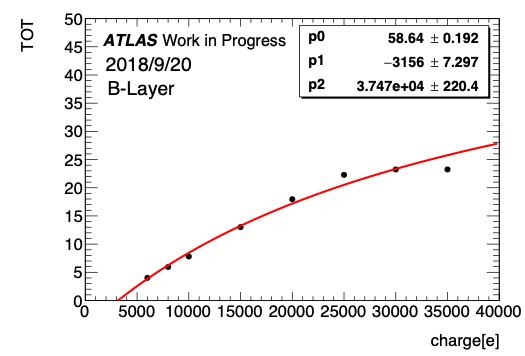
\includegraphics[keepaspectratio, scale=0.85]{calibhoseimae.png}
  \end{minipage}
  \begin{minipage}[b]{0.5\linewidth}
    \centering
    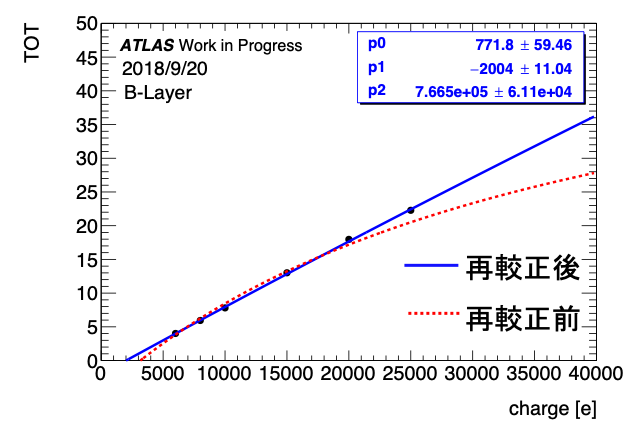
\includegraphics[keepaspectratio, scale=0.72]{calibhoseigo.png}
  \end{minipage}
  \caption[電荷再較正前後のフィッティング結果]{電荷再較正前(左図)と後(右図)のフィッティング結果。}
  \label{fig:calibhosei}
\end{figure}


%------------------------------------------------------------------------------------------------------------------------
\section{データに欠陥が含まれる場合の補完}
\label{sec:kessonhosei}
%------------------------------------------------------------------------------------------------------------------------
これまではピクセルモジュール内の一部のFEチップが欠陥しているデータがある場合には、最も近いFEチップから値をコピーすることにより補完していた。しかし、ピクセル検出器におけるモジュールは近いFEチップは2つまたは3つあるため、どの値を用いて補完を行うかは担当者の裁量によるものであった。より適切な方法を用いて自動処理を行うために、以下の二つの補完方法を導入する。
\begin{itemize}
  \item[1. ] 同一FEチップ上の他のピクセルタイプの平均値を用いた補完(\fref{fig:houhouhou}の左)
  \item[2. ] 欠陥している部分を除いた全てのFEチップの平均値を用いた補完(\fref{fig:houhouhou}の右)
\end{itemize}
各パラメータの補完のため、2つの補完方法の内、どちらがより実際の値を再現するかの評価を行った。

\begin{figure}[tbp]
  \begin{minipage}[b]{0.45\linewidth}
    \centering
    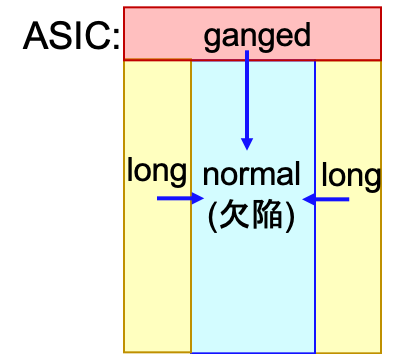
\includegraphics[keepaspectratio, scale=0.6]{houhousame.png}
  \end{minipage}
  \begin{minipage}[b]{0.55\linewidth}
    \centering
    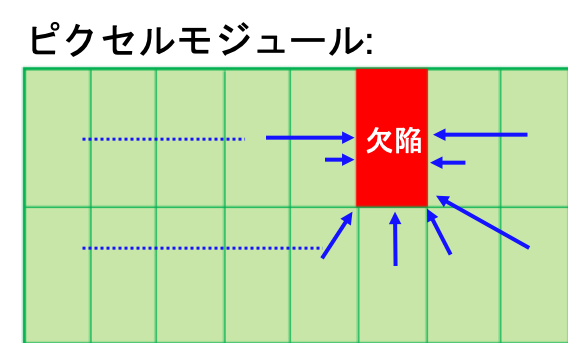
\includegraphics[keepaspectratio, scale=0.7]{houhoudiff.png}
  \end{minipage}
  \caption[データ欠陥の補完方法]{データ欠陥の補完方法についての概念図。左図はあるFEチップにおいて、normalピクセルの値が欠陥している場合に、longおよびgangedピクセルから補完することを示す。右図は欠陥の補完のために、異なるFEチップにある値を用いて補完することを示す。}
  \label{fig:houhouhou}
\end{figure}


%------------------------------------------------------------------------------------------------------------------------
\subsection{評価方法}
%------------------------------------------------------------------------------------------------------------------------
補完方法の評価のため、電荷較正結果に含まれるパラメータの1つが欠陥していると仮定し、そのパラメータと補完により得られる値の差を計算し分布の作成を行った。評価を行う際、2018年9月に行われた電荷較正の結果を用いた。IBLおよびピクセル検出器の全ての層について評価を行ったが、全ての層について同様の結果が得られたため、以下ではB-Layerの結果のみについての議論を行う。

%------------------------------------------------------------------------------------------------------------------------
\subsection{評価結果と考察}
%------------------------------------------------------------------------------------------------------------------------

前節において説明した方法を用いて、補完方法の評価を行った。\fref{fig:kekkanthreshold}はNormalピクセルにおけるThresholdについての評価結果を表す。この結果から、Threshold値は補完方法1の同一FEチップにおける別のピクセルタイプから得られる平均値を用いて補完した場合の方が、より精度良く補完を行うことがわかる。これはThresholdのチューニング方法によるものだと考えられる。チューニングではあるFEチップにおけるピクセル全体にglobalチューニングを行った後、各ピクセルごとにlocalチューニングを行う。初めにglobalチューニングを行うことから、別のFEチップの値を用いて補完するより、同一FEチップの値を用いて補完する方が実際の値に近い値を用いた補完を行うことができる。

\fref{fig:kekkannoise}はNormalピクセルにおけるThresholdのノイズについての評価結果を表す。この結果から、ノイズは補完方法2の別のFEチップにおける同一ピクセルタイプから得られる平均値を用いて補完した場合の方が、より精度良く補完を行うことができるとわかる。gangedピクセルはnormalピクセル2つをワイヤーで接続しているため、normalピクセルに比べてノイズが大きくなる。さらに、longピクセルは長方形の一片の長さがnormalピクセルの1.5倍あるため、normalピクセルと比べてピクセル間に生じるキャパシタンスが大きくなる。これによりFEチップ内の回路にノイズが加わり、longピクセルのノイズはnormalピクセルよりもノイズが大きくなる。


\begin{figure}[tbp]
  \begin{minipage}[b]{0.5\linewidth}
    \centering
    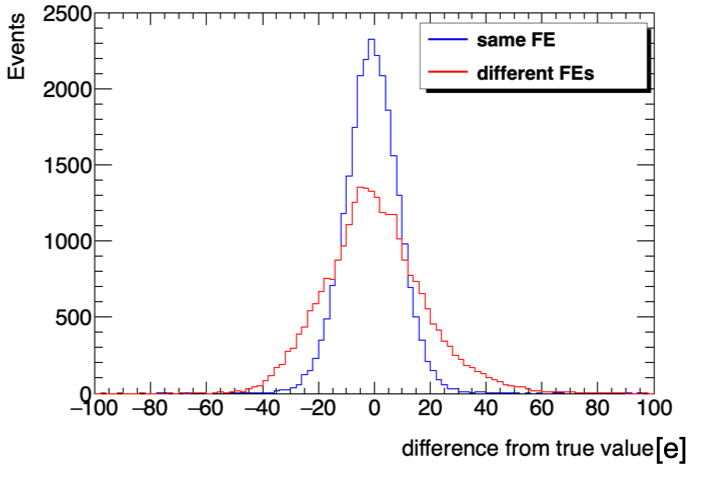
\includegraphics[keepaspectratio, scale=0.6]{kekkanthreshold.png}
    \caption[Thresholdの評価結果]{Thresholdの評価結果。同一FEチップにおける平均値の分布(青色)は、異なるFEチップの値の平均値の分布(赤色)よりのピークが鋭くなっている。}
    \label{fig:kekkanthreshold}
  \end{minipage}
  \begin{minipage}[b]{0.5\linewidth}
    \centering
    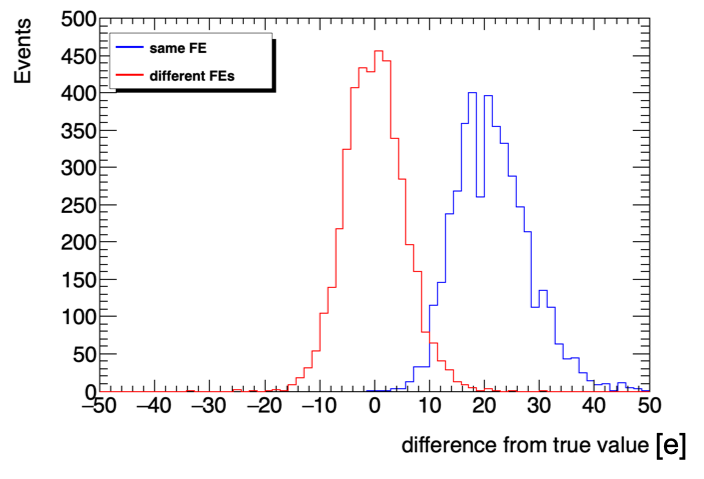
\includegraphics[keepaspectratio, scale=0.6]{kekkannoise.png}
    \caption[Thresholdのノイズの評価結果]{Thresholdのノイズの評価結果。同一FEチップの平均値の分布(青色)は、ピークの中心値がゼロからずれている。\\}
    \label{fig:kekkannoise}
  \end{minipage}
\end{figure}

他のパラメータについては\fref{fig:kekkannoise}と同様に、補完方法1と2の分布のピークの中心値が異なる結果が得られたため、補完方法2を用いることにより実際の値に近い値を再現できると考えられる。

%------------------------------------------------------------------------------------------------------------------------
\subsection{欠陥補完のための解析ツール}
%------------------------------------------------------------------------------------------------------------------------
上記の評価結果を用いて、自動で補完処理を行うツールの作成を行った。欠陥補完のための処理の流れを以下に示す。
\begin{itemize}
  \item[1. ] 補完結果のファイルを読み込む
  \item[2. ] 結果ファイル内の全てのモジュールについて、補完方法1および2を用いて値の補完を行う
  \item[3. ] スキャンが行われていないモジュールがあれば、一つ前の電荷較正結果の値をコピーし補完する
  \item[4. ] 補完結果をデータベースにアップロード可能なフォーマットに整形する
\end{itemize}

電荷較正結果をデータベースにアップロードするためには、電荷較正が行われていないモジュールの結果についても結果ファイル内に書き込む必要がある。そのため、処理の流れの3のように、電荷較正が行われていないモジュールについては1つ前の電荷較正結果から値をコピーすることにより補完を行う。また、データベースへアップロードするためには補完結果のファイルの中身を整形する必要があり、その処理についても補完処理を行うツールの最後に行う。

%------------------------------------------------------------------------------------------------------------------------
\section{自動補完のための解析ツール}
\label{sec:kaisekitool}
%------------------------------------------------------------------------------------------------------------------------
\ref{sec:calibhosei}節および\ref{sec:kessonhosei}節で示した補完方法を用いて自動で補完処理を行う解析ツールの開発を行った。解析ツールが行う処理の流れを以下に示す。

\begin{itemize}
  \item[1. ] \fref{fig:saikouseiflow}の流れで電荷較正および再較正
  \item[2. ] CERNのデータベースにアクセスし、1つ前の電荷較正結果の履歴を取得
  \item[3. ] \ref{sec:kessonhosei}節に示した解析ツールを用いて欠陥の補完および結果ファイルの整形
  \item[4. ] 補完についてのまとめファイルを出力
\end{itemize}

処理の流れの4番目に示すように、電荷再較正および欠陥の補完を行った後にどの様に補完を行ったかについてのまとめファイルを出力する。まとめファイルの例を\cref{code:matomefile}に示す。まとめファイルのはじめに、どのように補完が行われるかを記し、その後に補完結果が確認できる様にした。

\begin{lstlisting}[caption=解析ツールにより出力される補完結果のまとめ,label=code:matomefile, language=C++]
##===========================================================================
## This file shows the way to recover data loss and calibration failure.
##
## How to recover parameters:
## 1. If there is a data loss in output data:
##   - Case1: Partial loss in a module
##     - Threshold: Recover using average of same FE
##     - Others:    Recover using average of different FEs
##   - Case2: All values loss in a module
##     - Previous scan result is used for the recovery
##
## 2. If there is a calibration failure:
##   - Remove incorrect injected charge & refitting
##   - Removed charges are listed in order of deletion
##
## Example of an output for a module:
##   L0_B08_S1_A6_M2A:
##   I2: [ normal threshold ], [ ] <--- Parameters that become '0' is listed
##   I8: [ ], [ 30000 40000 ] <-------- Injected charges that removed is listed
##
##===========================================================================

~~~~~~~~ Summary for the recovery ~~~~~~~~
1. Number of parameters that were 0
Number of FEs with all values zero: 11
normal threshold: 11
normal noise: 11
normal sigma: 11
normal intime: 27
fit_normal A: 11
fit_normal E: 11
fit_normal C: 11
quality/unused unused: 11
quality/unused fit_quality: 11

2. Number of FEs that had bad fits
B-Layer: 0
Layer1: 0
Layer2: 0
Disk: 5

3. Number of modules that were not scanned
B-Layer: 286
Layer1: 494
Layer2: 676
Disk: 6
~~~~~~~~~~~~~~~~~~~~~~~~~~~~~~~~~~~~~~~~~~

D1A_B01_S1_M1:
I0 [ normal threshold ], [ ]
D1A_B01_S1_M2:
D1A_B01_S1_M3:
I8: [ ], [ 30000 40000 ]
\end{lstlisting}



%------------------------------------------------------------------------------------------------------------------------
\section{解析ツールの運用}
\label{sec:unnyou}
%------------------------------------------------------------------------------------------------------------------------

RUN3におけるATLAS実験のためのモンテカルロシミュレーションのサンプル作成のために、2021年9月に電荷較正のためのデータ取得が行われた。電荷較正結果をデータベースにアップロードするために、本研究で作成した解析ツールを用いて電荷較正結果を作成した。以下では、電荷較正における補完結果をまとめる。


%------------------------------------------------------------------------------------------------------------------------
\subsection{補完のまとめ}
\label{sec:matome}
%------------------------------------------------------------------------------------------------------------------------
電荷較正結果と同時に出力されるファイルを用いて、補完内容の確認を行なった。\tref{tab:hokannmatome}に補完結果のまとめを示す。この結果から、各モジュールに存在した欠陥を取り除き、値の再現ができたと考えられる。次節において、電荷較正についての詳細を示す。

\begin{table}[htbp]
  \begin{center}
    \caption[RUN3に向けた電荷較正補完のまとめ]{RUN3に向けた電荷較正補完のまとめ。}
    \label{tab:hokannmatome}
    \begin{tabular}{|l||c|c|c|c|}
    \hline
      補完項目 & B-Layer & Layer1 & Layer2 & Disk  \\
    \bhline{1.5pt}
      スキャンされなかったモジュール数  & 14 & 18 & 40 & 6 \\
    \hline
      欠陥していたFEチップの数  & 18 & 46 & 38 & 11 \\
    \hline
      部分的に0となっていたパラメータ数  & 0 & 6 & 8 & 3 \\
    \hline
      再較正を行なったFEチップの数 & 179 & 1 & 9 & 5 \\
    \hline
    \end{tabular}
  \end{center}
\end{table}


%------------------------------------------------------------------------------------------------------------------------
\subsection{RUN3での電荷再較正}
\label{sec:saisinsaikousei}
%------------------------------------------------------------------------------------------------------------------------
\fref{fig:blayernew}に2021年9月に行われたB-Layerについての電荷較正のフィッティング結果の例を示す。\fref{fig:blayernew}に示すように、電荷較正では2つの構造が確認できた。

\begin{figure}[tbp]
  \begin{minipage}[b]{0.5\linewidth}
    \centering
    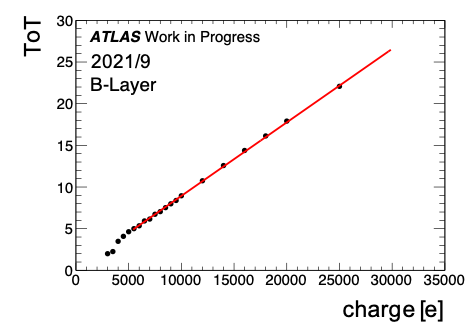
\includegraphics[keepaspectratio, scale=0.8]{blayernew1.png}
  \end{minipage}
  \begin{minipage}[b]{0.5\linewidth}
    \centering
    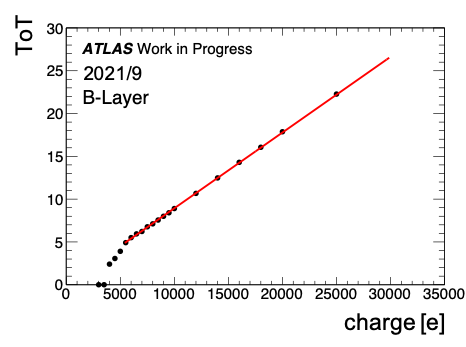
\includegraphics[keepaspectratio, scale=0.8]{blayernew2.png}
  \end{minipage}
  \caption[2021年9月に行われたB-Layerについての電荷較正結果]{2021年9月に行われたB-Layerについての電荷較正結果。}
  \label{fig:blayernew}
\end{figure}

\fref{fig:blayernew}の左図は、Threshold値に近い小さい試験電荷量の点についてもToTから電荷量が再現できるものである。B-Layerではデジタル回路のThresholdとは別に、ToTの閾値が$3\ \si{ToT}$と定義されている。そのため、ToTが4以上であればデータの取得を行うが、そのようなものについても正しく較正できる。

一方で、\fref{fig:blayernew}の右図は、Threshold値に近い小さい試験電荷量の点についてToTから電荷量の較正が正しくできないものである。ToTが5以上であれば、試験電荷から得られる点のフィット曲線上にあるため正しく較正できるが、$\mathrm{ToT}=4$の場合は、正しく較正できなくなってしまう。

RUN2終了時までの電荷較正では電荷較正に用いられる試験電荷の最小値は$6000\ \si{e}$であり、電荷量を$2000\ \si{e}$ずつ変化させてデータの取得を行っていたため小さい試験電荷についての2つの構造が確認できていなかった。しかし、RUN3に向けた電荷較正では、放射線損傷による電荷収集の低下を保障するようThresholdを$3500\ \si{e}$まで引き下げられた。さらに、試験電荷の電荷量は$500\ \si{e}$ずつ変化させスキャンを行うため、このような違いが確認できるようになったと考えられる。そのため、小さい試験電荷を用いたToTスキャンについての理解を深め、\fref{fig:blayernew}の右図のような電荷較正結果が得られた際の電荷較正手法について再検討する必要があると考える。


\newpage
